\chapter{2023/10/16}\label{20231016}

\section{Something about dimension analysis and Planck units
一些关于量纲分析和普朗克单位的内容}\label{something-about-dimension-analysis-and-planck-units-ux4e00ux4e9bux5173ux4e8eux91cfux7eb2ux5206ux6790ux548cux666eux6717ux514bux5355ux4f4dux7684ux5185ux5bb9}

\subsection*{(1) Einstein radius
爱因斯坦角半径}\label{einstein-radius-ux7231ux56e0ux65afux5766ux89d2ux534aux5f84}

The Einstein radius, \(\theta_E\), is the radius of an Einstein ring,
and \[\theta_E = \sqrt{4GM \over c^2 \cdot D_r},\] where \(D_r\) is the
\emph{impact parameter} (the distance of nearest approach of the
lightbeam to the center of mass).

\subsection*{(2) Planck charge
普朗克电量}\label{planck-charge-ux666eux6717ux514bux7535ux91cf}

From the fine structure constant \(\alpha = \dfrac{e^2}{\hbar c}\)
(under \(\text{cgs}\) system), we can see that \[[e^2] = [\hbar c].\]
Therefore, we can define the Planck charge \[e_P = \sqrt{\hbar c}.\]

\section{Gauge transformation (by Hermann Weyl)
规范场变换}\label{gauge-transformation-by-hermann-weyl-ux89c4ux8303ux573aux53d8ux6362}

From the second equation of the Maxwell's equations \[\nabla \cdot \boldsymbol B = 0,\] we can see \(B\) as the curl of a certain vector \(\boldsymbol A\). We call this \(\boldsymbol A\)
\textbf{magnetic vector potential} (磁矢势), and
\[\boldsymbol B  = \nabla \times \boldsymbol A.\]

Because the curl of the gradient of a certain scalar (标量梯度的旋度) is zero, we can add the gradient of a scalar field \(\psi\): \[\boldsymbol A \mapsto \boldsymbol A + \nabla \psi, \quad  (*)\] and we get \[\boldsymbol B  = \nabla \times (\boldsymbol A + \nabla \psi).\]

Substitute \(\boldsymbol B\) in
\[\nabla \times \boldsymbol E = -{\partial \boldsymbol B \over \partial t},\]
and we can get
\[\nabla \times \boldsymbol E = - {\partial \over \partial t} \left( \nabla \times \boldsymbol A \right) = - \nabla \times {\partial \boldsymbol A \over \partial t}\]
\[\nabla \times \left(\boldsymbol E + {\partial \boldsymbol A \over \partial t} \right) = \boldsymbol 0.\]

From this, we can see
\(\boldsymbol E + \dfrac{\partial \boldsymbol A }{ \partial t}\) as the
negative of the gradient of a scalar field \(\varphi\) (标量场
\(\varphi\) 梯度的负), and
\[\boldsymbol E = - \dfrac{\partial \boldsymbol A }{ \partial t} - \nabla \varphi.\]

When we put in the \(\boldsymbol A\) shown by \((*)\), we can get:
\begin{align*}
    \boldsymbol E & = - \dfrac{\partial}{ \partial t}(\boldsymbol A + \nabla \psi) - \nabla \varphi \\
    & = - \dfrac{\partial \boldsymbol A }{ \partial t} - \nabla \left(\varphi + {\partial \psi \over \partial t}\right).
\end{align*}

This shows that, when we make the transformation below (\textbf{the gauge transformation} 规范变换) \[\left\{
    \begin{array} {l}
        \boldsymbol A \mapsto \boldsymbol A + \nabla \psi; \\
        \varphi \mapsto \varphi - \dfrac{\partial \psi}{\partial t}.
    \end{array}
\right.\]

We can ensure that the fields \(\boldsymbol B\) and \(\boldsymbol E\)
remain unchanged.

\section{The Kronecker Delta
克罗尼克符号}\label{the-kronecker-delta-ux514bux7f57ux5c3cux514bux7b26ux53f7}

We define the Kronecker Delta in this way: \[\delta_{ij} = \left\{
    \begin{aligned}
        1,\ \ &i = j \\
        0,\ \ &i \neq j
    \end{aligned}
\right.\]

Example of practical use:
\[\boldsymbol a \cdot \boldsymbol b = (a_i \boldsymbol e_i) \cdot (b_j \boldsymbol e_j) = a_ib_j \delta_{ij}.\]

\section{The Levi-Civita Symbol
列维-奇维塔符号}\label{the-levi-civita-symbol-ux5217ux7ef4-ux5947ux7ef4ux5854ux7b26ux53f7}

We define the Levi-Civita Symbol in this way:
\[\boldsymbol e_i \times \boldsymbol e_j = \varepsilon_{ijk} \boldsymbol e_k.\]
In other words, \[\varepsilon_{ijk} = \left\{
    \begin{aligned}
        1, & \ \ &\text{even permutation (偶置换)};  \\
        -1, & & \text{odd permutation (奇置换)};\\
        0, & & i=j \ \text{or} \ i = k \ \text{or} \ j = k \ \text{(有重合指标)}.
    \end{aligned}
\right.\]

In the following picture, the left is for even permutations, and the
right for odd permutations:

\begin{center}
    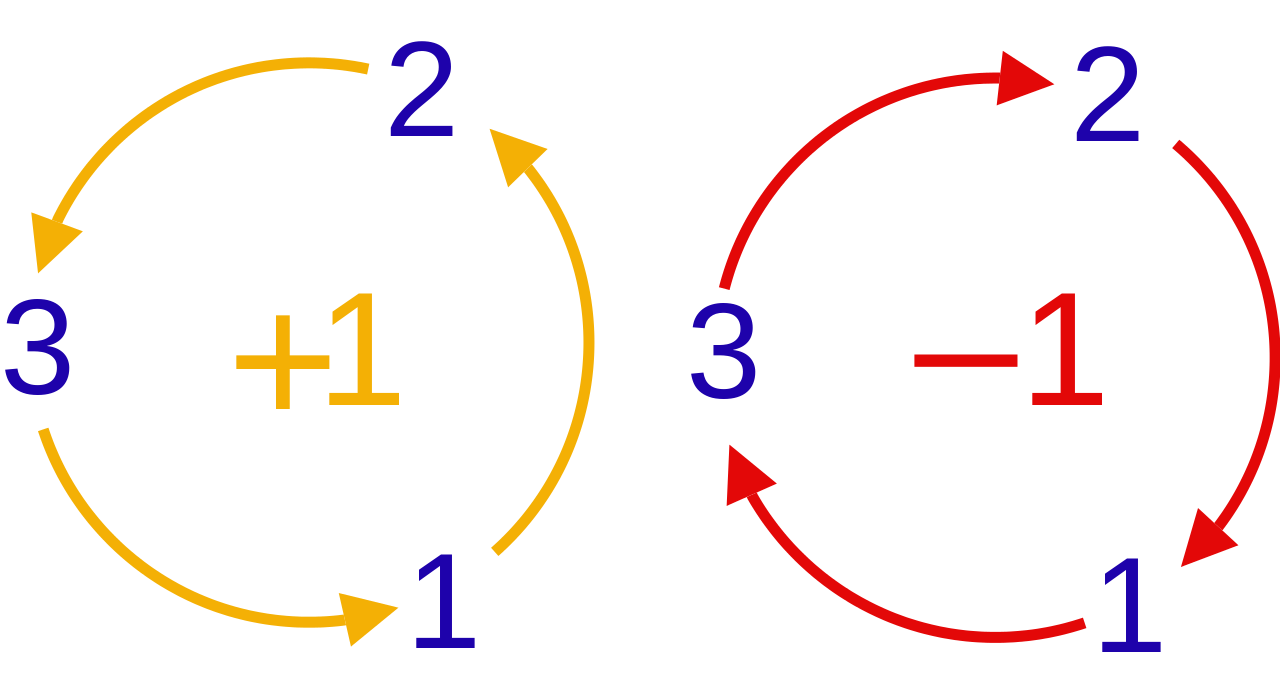
\includegraphics[height=80pt]{assets/Levi-Civita_Symbol.png}
    \captionof{figure}{Levi-Civita symbol (Source: Wikipedia)}
\end{center}

In word form, if \((i,j,k)\) is \((1,2,3)\), \((2,3,1)\) or \((3,1,2)\),
then \(\varepsilon_{ijk} = 1\). If \((i,j,k)\) is \((3,2,1)\),
\((1,3,2)\) or \((2,1,3)\), then \(\varepsilon_{ijk} = -1\).

Example of practical use:
\[\boldsymbol a \times \boldsymbol b = (a_i \boldsymbol e_i) \times (b_j \boldsymbol e_j) = a_ib_j \varepsilon_{ijk} \boldsymbol e_k.\]

\section{Einstein summation convention
爱因斯坦求和约定}\label{einstein-summation-convention-ux7231ux56e0ux65afux5766ux6c42ux548cux7ea6ux5b9a}

In this notation (标记法), when an index variable appears twice in a
single term and is not otherwise defined, it implies summation of that
term over all the values of the index.

For example, if index \(i\) ranges over the set \(\{1, 2, 3\}\), then \(y = c_ix^i\) means \[y = \sum_{i=1}^3 c_ix_i = c_1x_1 + c_2x_2 + c_3x_3.\]

An index that is summed over is a \textbf{summation index}, in this case
\(i\). It is also called a \textbf{dummy index (哑标)} since any symbol can
replace \(i\) without changing the meaning of the expression (provided
that it does not collide with other index symbols in the same term).

An index that is not summed over is a \textbf{free index} (自由指标) and
should appear only once per term. If such an index does appear, it
usually also appears in every other term in an equation. An example of a
free index is the \(i\) in the equation \(v_i = a_i b_j x^j\), which is
equivalent to the equation \(v_i = \sum_j(a_i b_j x^j)\).

Examples:

\subsection*{(1) Lorentz force}\label{lorentz-force}

\[\boldsymbol F = q(\boldsymbol E + \boldsymbol v \times \boldsymbol B)\]
\[F_k = q (E_k + v_i B_j \varepsilon_{ijk})\]

Dummy indices \(-\) \(i\), \(j\); Free index \(-\) \(k\)

\subsection*{(2) Maxwell's equations}\label{maxwells-equations}

\[\left\{
    \begin{aligned}
        &\dfrac{\partial E_i}{\partial x^i} = \dfrac{\rho}{\varepsilon_0} & \ \ &  i \text{ -- Dummy index}\\
        &\dfrac{\partial B_i}{\partial x^i} = 0 && i \text{ -- Dummy index}\\
        &\dfrac{\partial E_j}{\partial x_i}\varepsilon_{ijk} = - \dfrac{\partial B_k}{\partial t} && i, j \text{ -- Dummy indices;} \ k \text{ -- Free index}\\
        &\dfrac{\partial B_j}{\partial x_i}\varepsilon_{ijk} = \mu_0\left( j_k + \varepsilon_0\dfrac{\partial E_k}{\partial t}\right) && i, j \text{ -- Dummy indices;} \ k \text{ -- Free index}
    \end{aligned}
\right.\]
